\documentclass{beamer}

\usepackage{amsmath,amssymb}
\usepackage{color}
\usepackage[UTF8,noindent]{ctexcap}
\usepackage{textcomp}
%\usepackage[timeinterval=1]{tdclock}%显示当前时间宏包
%%\usetheme{AnnArbor}
%\usetheme{Antibes}
%\usetheme{CambridgeUS}
%\usetheme{Copenhagen}
%\usetheme{Darmstadt}%!
%\usetheme{Dresden}
%\usetheme{Frankfurt}%!!
%\usetheme{Goettingen}
%\usetheme{Hannover}
%\usetheme{Ilmenau}
%\usetheme{JuanLesPins}
%\usetheme{Luebeck}
%\usetheme{Madrid}
%\usetheme{Marburg}
%\usetheme{PaloAlto}%!
%\usetheme{Singapore}
\usetheme{Warsaw}

%\usetheme{Warsaw}%\usetheme{Copenhagen}%\usetheme{CambridgeUS}%\usetheme{Ilmenau}%\usetheme{AnnArbor}%\usetheme[secheader]{Boadilla}
%\useoutertheme[subsection=false]{miniframes}
%\useinnertheme{circles}
%\usecolortheme{seahorse}
%\usefonttheme{serif}
%在该文件控制主题样式
%\usetheme{Warsaw}
\usetheme{Frankfurt}
%\usetheme{Copenhagen}
%\usetheme{CambridgeUS}
%\usetheme{Ilmenau}
%\usetheme{AnnArbor}
%\usetheme[secheader]{Boadilla}
%\useoutertheme[subsection=false]{miniframes}
%\useinnertheme{circles}
%\usecolortheme{seahorse}
%\usefonttheme{serif}
%\usetheme{Warsaw}
\setbeamertemplate{caption}[numbered]%给beamer加编号
%\usepackage{cases}
\renewcommand{\rmdefault}{ptm}
\AtBeginSection[]{%设置每section前生成当前目录
\begin{frame}{本节目录}
\tableofcontents[currentsection]
\end{frame}
}

\title[混沌系统的Koopman分析与应用]{\LARGE 混沌系统的Koopman分析与应用}
\subtitle{复杂系统的边界点划分}
\author{张聪}
\institute[北京邮电大学理学院(系统科学)]{指导教师:兰岳恒\\北京邮电大学理学院}
\date[理学硕士学位论文答辩]{理学硕士学位论文答辩\\2020-09-30}
\logo{
\includegraphics[scale=0.08]{figure/bupt_logo.jpg}}

\begin{document}
\kaishu

\begin{frame}
\titlepage
\end{frame}

\begin{frame}{目录}
\tableofcontents[pausesections]
\end{frame}

\section{研究背景与意义}
		\begin{frame}{研究背景与意义}
		\begin{block}{研究背景}
		\begin{enumerate}
			\item 信息时代\textrightarrow 信息\textrightarrow 数据 \textrightarrow 数据分析
			\item 动力学系统\textrightarrow 线性、非线性
			\item 非线性动力学
			\item 动力学系统的数值计算
			\item Koopman算符→提取系统的关键特征
		\end{enumerate}
		\end{block}
		\begin{block}{意义:通过Koopman算符分析系统关键特征}
\indent 我们希望能够找到一种方法,仅通过系统数据的演化过程得到系统的一些演化特征,并在这些演化特征中提取出关键特征。Koopman算符给我们提供了一个有效的数学工具。Koopman算法由B.O.Koopman与1931年引入,它作用在某个函数上,描述了函数的演化。若将系统的特性数据演化视为函数的演化,我们即可以用Koopman算符分析系统的特征。
		\end{block}
		\end{frame}
		
\section{Koopman算符介绍}
	\subsection{定义}
	\begin{frame}{Koopman算符}
	\begin{block}{Koopman算符定义}
		$$Uf\left( x\right)=f\left(T\left( x\right)\right)=\tilde{f}\left( x\right)$$
		对于固定的时间t,上式可写为
		$$U_tf\left( x\right)=f\left(T_t\left( x\right)\right)=\tilde{f}_t\left( x\right)$$
	\end{block}
	\begin{block}{举例}
	对于一个函数:$f(x)=x^2$\\
	动力学方程:$\dot{x}=-2x \rightarrow x(t)=x(0)e^{-2t} \rightarrow T_t(x)=xe^{-2t}$\\
	Koopman算符:$U_tf(x)=f(T_t(x))=f(xe^{-2t})=x^2e^{-4t}=\tilde{f}(x)$
	\end{block}
	\begin{itemize}
		\item 	\textcolor{red}{Koopman算符描述了函数的演化}
	\end{itemize}
	\end{frame}
	\subsection{Koopman算符的本征函数}
	\begin{frame}{Koopman算符在函数空间上的描述}
	对于一个可观测量函数$f(x)$,自变量经过时间t的演化变为$\tilde{f}(x)$
	$$f(x)\xrightarrow{t}\tilde{f}(x)$$
	用Koopman算符可表示为
	$$Uf(x_p)=f(x_{p+1})=\tilde{f}(x_p)$$
	其中p表示时间因子,在m维函数空间中将可观测量展开
	$$f(x_p)=\sum_{i=1}^{m}\alpha_ig_i(x_p)$$
	则
	$$Uf(x_p)=\sum_{i=1}^{m}\alpha_iUg_i(x_p)=\sum_{i=1}^{m}\alpha_i\tilde{g}_i(x_p)=\tilde{f}(x_p)$$
	$$Uf(x_p)=\sum_{i=1}^{m}\alpha_ig_i(x_{p+1})=f(x_{p+1})$$
	\end{frame}
	\begin{frame}{Koopman算符的本征值和本征函数}
	\begin{block}{本征函数的定义}
		$$U\phi _k(x)=\phi _k(T(x))=\lambda _k\phi _k(x)$$
	\end{block}
	在函数空间中
	$$\phi (x)=\sum_{i=1}^{m}a_ig_i(x)$$
	$$U\phi (x)=\sum_{i=1}^{m}a_iUg_i(x)=\sum_{i=1}^{m}a_i\tilde{g}_i(x)$$
	$$U\phi(x)=\lambda (x)=\sum_{i=1}^{m}\lambda a_ig_i(x)$$
	\end{frame}
	\begin{frame}{本征函数的性质}
		根据本征函数的定义,我们有
		$$\phi_k(x_p)=U\phi_k(x_{p-1})=\lambda \phi_k(x_{p-1})=\cdots=\lambda^p\phi_k(x_0)$$
		当$\lambda=1$时,$$\phi_k(x_p)=\phi_k(x_{p-1})=\cdots=\phi_k(x_0)$$
		\begin{itemize}
			\item 本征值$\lambda=1$下的本征函数中,函数值相等的点属于一个不变集。
			\item 在动力学系统中,不变集与不动点和周期轨道密切相关
		\end{itemize}
	\end{frame}
	\begin{frame}{Koopman算符的本征函数的计算}
	Koopman算符作用在一组基函数上可得到一组基函数的演化,即
	$$U(g_1(x),g_2(x),\cdots,g_m(x))=(\tilde{g}_1(x),\tilde{g}_2(x),\cdots,\tilde{g}_m(x))$$
	简记为$$UK=L$$
	其中
	\tiny
	\begin{gather}
	K=(g_1(x_p),g_2(x_p),\cdots,g_m(x_p))=
	\begin{pmatrix}
	g_1(x_{p_1})&g_2(x_{p_1})&\cdots&g_m(x_{p_1})\\
	g_1(x_{p_2})&g_2(x_{p_2})&\cdots&g_m(x_{p_2})\\
	\vdots&\vdots&\ddots&\vdots\\
	g_1(x_{p_n})&g_2(x_{p_n})&\cdots&g_m(x_{p_n})
	\end{pmatrix}\\
	L=(\tilde{g}_1(x_p),\tilde{g}_2(x_p),\cdots,\tilde{g}_m(x_p))=
	\begin{pmatrix}
	\tilde{g}_1(x_{p_1})&\tilde{g}_2(x_{p_1})&\cdots&\tilde{g}_m(x_{p_1})\\
	\tilde{g}_1(x_{p_2})&\tilde{g}_2(x_{p_2})&\cdots&\tilde{g}_m(x_{p_2})\\
	\vdots&\vdots&\ddots&\vdots\\
	\tilde{g}_1(x_{p_n})&\tilde{g}_2(x_{p_n})&\cdots&\tilde{g}_m(x_{p_n})
	\end{pmatrix}\\
	L=(g_1(x_{p+1}),g_2(x_{p+1}),\cdots,g_m(x_{p+1}))=
	\begin{pmatrix}
	g_1(x_{p_1+1})&g_2(x_{p_1+1})&\cdots&g_m(x_{p_1+1})\\
	g_1(x_{p_2+1})&g_2(x_{p_2+1})&\cdots&g_m(x_{p_2+1})\\
	\vdots&\vdots&\ddots&\vdots\\
	g_1(x_{p_n+1})&g_2(x_{p_n+1})&\cdots&g_m(x_{p_n+1})
	\end{pmatrix}
	\end{gather}
	\end{frame}
	\begin{frame}{Koopman分析的步骤}
	\begin{enumerate}
		\item 获得系统的特征数据$x_p$,$x_{p+1}$
		\item 选取合适的基函数空间$g(x)$(基函数形式、函数格点、演化格点)
		\item 确定某时刻的数据矩阵K及演化之后的数据矩阵L
		\item 通过$UK=L$计算出Koopman算符的矩阵表示
		\item 计算出Koopman算符的本征值$\lambda$和$\phi(x)$
		\item 找到我们关心的$\lambda$和$\phi(x)$(如$|\lambda|=1$)
		\item 系统特征分析
	\end{enumerate}
	\end{frame}
	\subsection{常见的混沌系统}
		\subsubsection{一维映射:Logistic Map}
		\begin{frame}{Logistic Map}
		\begin{block}{动力学方程}
			$$x_{n+1}=f(x_n)=\gamma x_n(1-x_n)$$
			$$x_n\in [0,1], n=1,2,3,\cdots$$
		\end{block}
		这里我们取$\gamma=4$,使该系统处于混沌状态。\\
		两个不动点:0和$\frac{3}{4}$。
		\begin{figure}
			\begin{minipage}{0.4\linewidth}
				\centering
				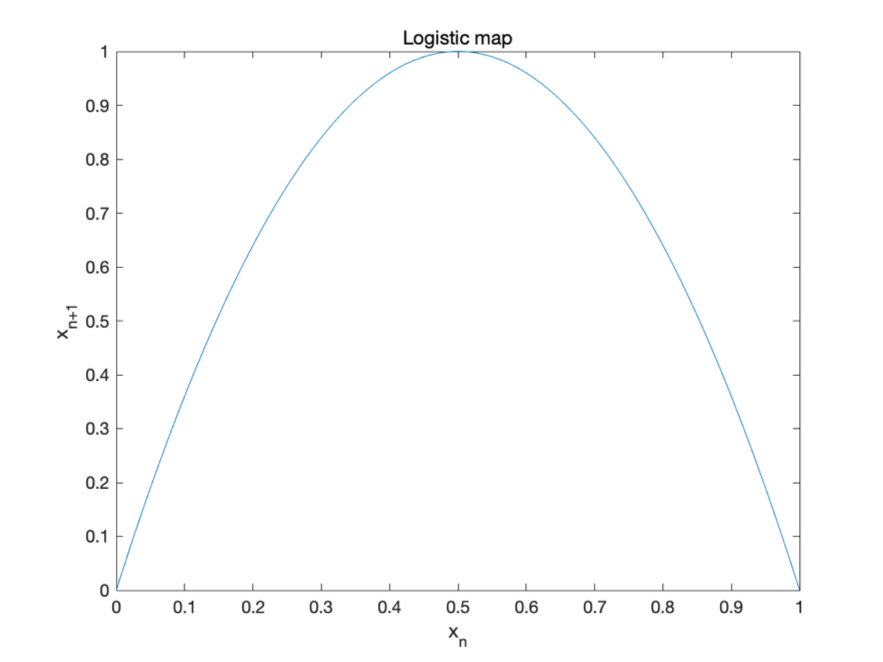
\includegraphics[width=1.8in]{figure/logistic_phase}
				\caption{Logistic map相图}
			\end{minipage}
			\begin{minipage}{0.4\linewidth}
				\centering
				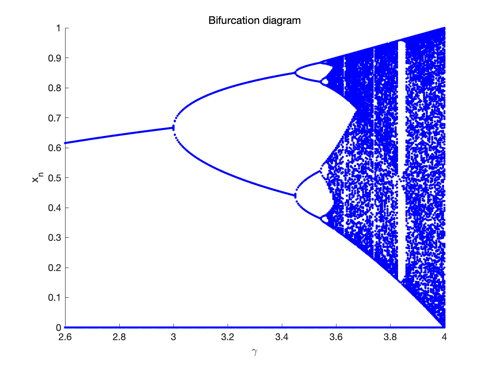
\includegraphics[width=1.8in]{figure/logistic_bifurcation}
				\caption{Logistic map分岔图}
			\end{minipage}
		\end{figure}
		\end{frame}
		\subsubsection{一维映射:Tent Map}
		\begin{frame}{Tent Map}
		\begin{block}{动力学方程}
			$$x_{n+1}=f(x_n)=1-2|x-\frac{1}{2}|$$
			$$x_n\in [0,1], n=1,2,3,\cdots$$
		\end{block}
		两个不动点:0和$\frac{2}{3}$
		\begin{figure}
			\begin{minipage}{0.4\linewidth}
				\centering
				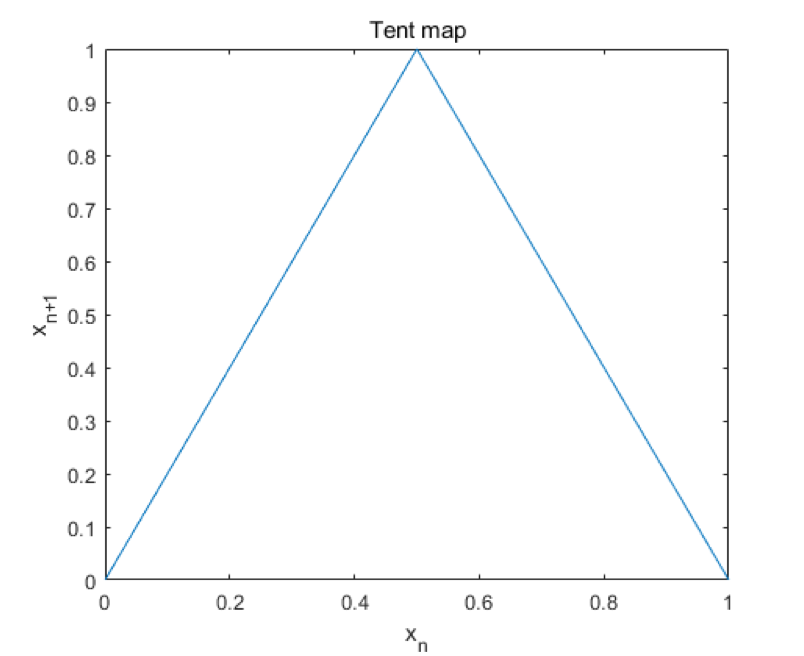
\includegraphics[width=1.8in]{figure/tent_phase}
				\caption{Tent map相图}
			\end{minipage}
		\end{figure}
		\end{frame}
		\subsubsection{二维映射:Henon Map}
		\begin{frame}{Henon Map}
		\begin{block}{动力学方程}
			\centering
			\begin{math}
			\begin{cases}
				x_{n+1}=y_n+1-ax_n^2\\
				y_{n+1}=bx_n
			\end{cases}\ x,y\in [-1.5,1.5]
			\end{math}
		\end{block}
		我们选取a=1.4,b=0.3使其处于混沌状态。\\
		两个不动点:(0.6314,0.1894)
和(-1.1314,-0.3394)
		\begin{figure}
			\begin{minipage}{0.4\linewidth}
				\centering
				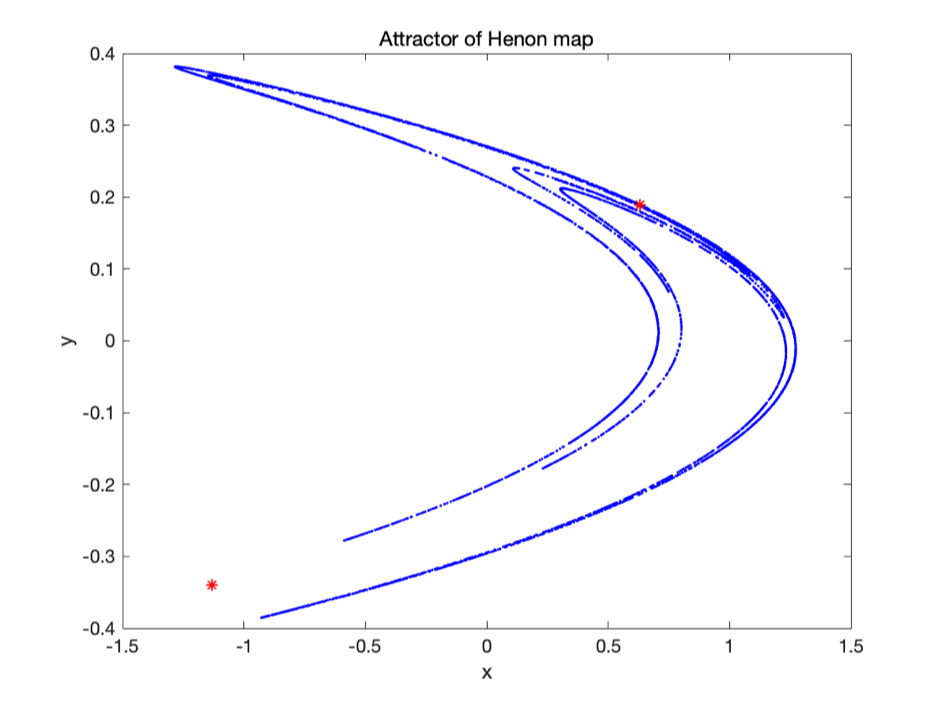
\includegraphics[width=1.8in]{figure/henon_phase}
				\caption{Henon map相图}
			\end{minipage}
		\end{figure}
		\end{frame}
		\subsubsection{三维流:Lorenz System}
		\begin{frame}{Lorenz System}
		\begin{block}{动力学方程}
			\centering
			\begin{math}
			\begin{cases}
			\dot{x}=\sigma (y-x)\\
			\dot{y}=x(\gamma-z)-y\\
			\dot{z}=xy-\beta z
			\end{cases}\
			\end{math}
		\end{block}
		取$\beta=\frac{8}{3}$,$\rho=28$,$\sigma=10$使系统处于混沌状态,初始点(-1,3,4)\\
		三个不动点:(0,0,0)
、(-8.4853,8.4853,27)
、(8.4853,-8,4853,27)
		\begin{figure}
			\begin{minipage}{0.4\linewidth}
				\centering
				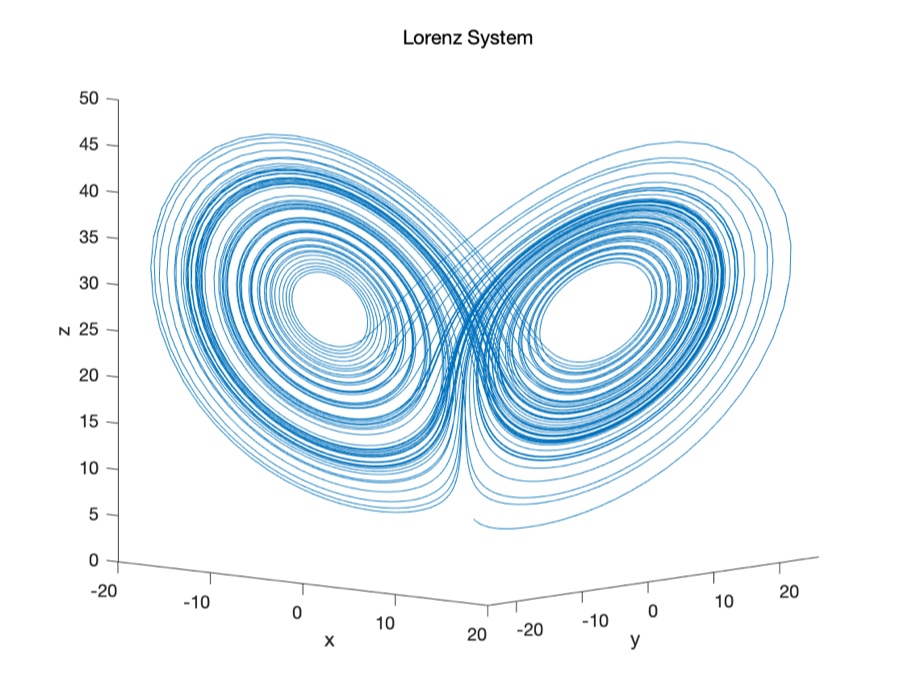
\includegraphics[width=1.6in]{figure/lorenz_phase}
				\caption{Lorenz System相图}
			\end{minipage}
		\end{figure}
		\end{frame}
\section{进展情况总结}
\begin{frame}{进展总结}
\begin{enumerate}
	\item Koopman算符提供了一个有效的数学工具,作用于某个函数并描述了该函数的演化。
	\item 若将系统特征数据的演化看作为相空间的函数的演化,则可以用Koopman算符分析系统的演化特征,进一步提取关键特性,并在一定程度上预测系统的长期行为。
	\item 本征函数值相等的点属于一个不变集。在动力学系统中,不变集与周期轨道密切相关。
	\item Koopman算符本征函数值的“极值点”在某些情况下与系统的“边界点”非常吻合。“边界点”反映了动力学系统的符号动力学划分,而符号动力学的划分可以预测系统的长期行为。
	\item 适用于任何动力学系统
\end{enumerate}
\end{frame}
\section{阶段性工作成果汇报:Koopman算符与相空间的划分}
\begin{frame}{Logistic map的本征函数(m=6)}
\begin{figure}
	\centering
	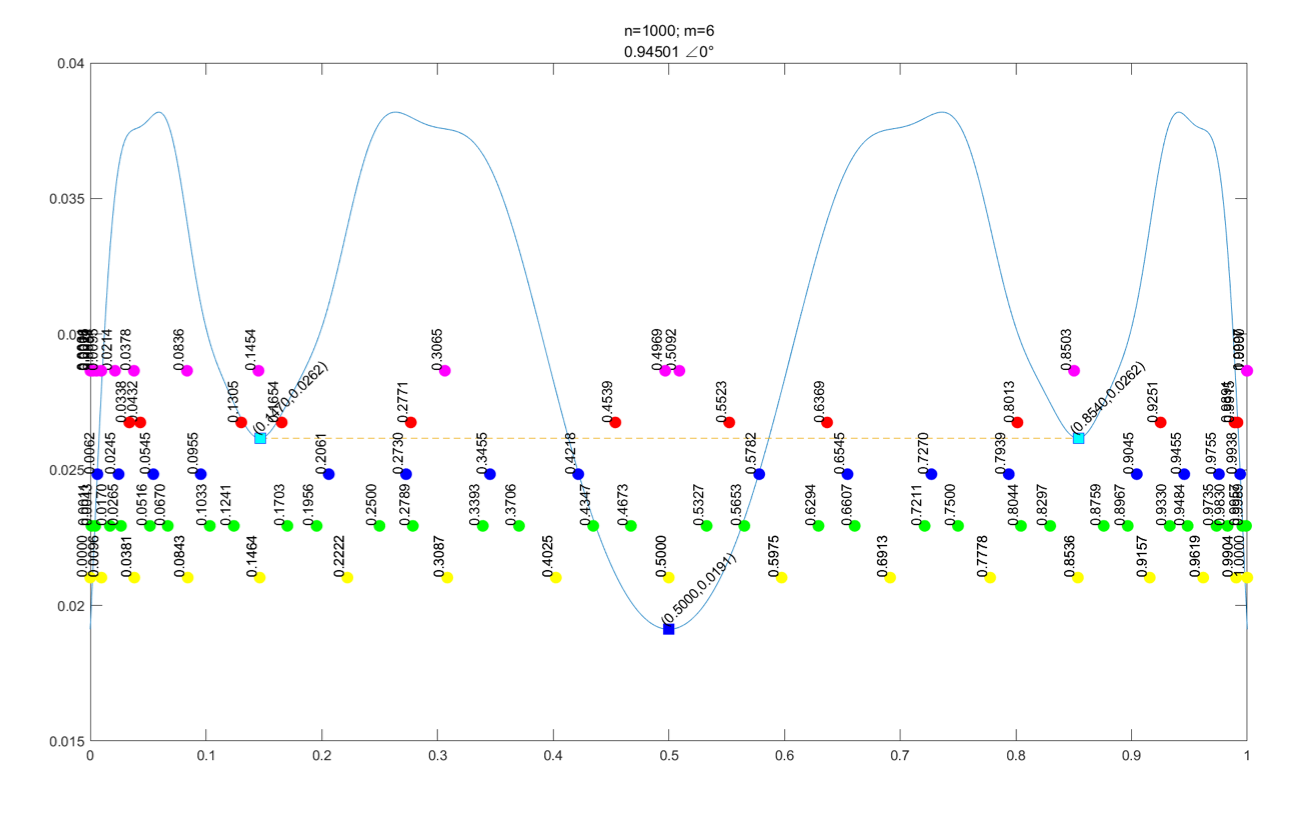
\includegraphics[width=3in]{figure/logistic_eigen_m6}
	\caption{Logistic map的本征函数(m=6)}
\end{figure}
可见,Koopman算符的极值点与动力学系统的“边界点”得到了较好的吻合。而边界点反映了Logistic Map的符号动力学。符号动力学的划分可以一定程度的预测系统的长期行为。
\end{frame}

\begin{frame}{符号动力学}
\begin{figure}
	\centering
	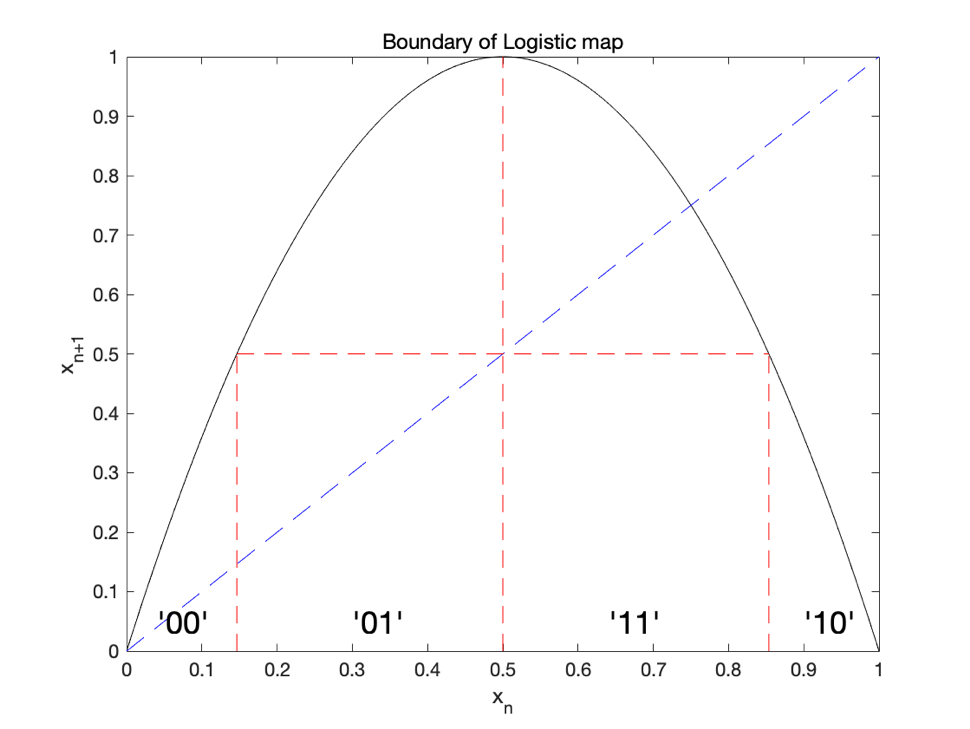
\includegraphics[width=3in]{figure/logistic_symbolic}
	\caption{Logistic Map的符号动力学划分}
\end{figure}
\begin{itemize}
	\item 相空间的任何一点都可以用一个符号动力学序列来表示
\end{itemize}
\end{frame}

\begin{frame}{Logistic map的本征函数(m=100)}
\begin{figure}
	\centering
	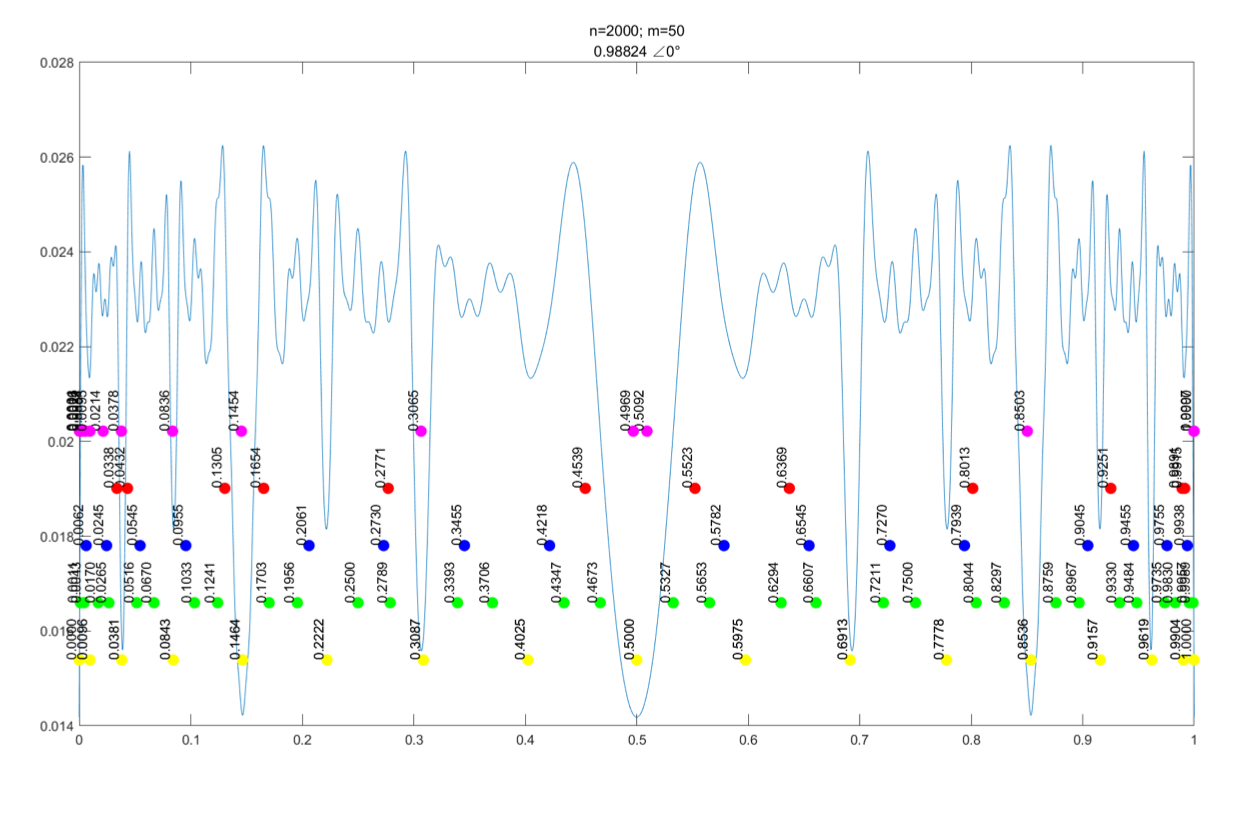
\includegraphics[width=3in]{figure/logistic_eigen_m100}
	\caption{Logistic map的本征函数(m=100)}
\end{figure}
\begin{itemize}
	\item Koopman算符的极值点与动力学系统的“边界点”得到了较好的吻合。而边界点反映了Logistic Map的符号动力学。符号动力学的划分可以一定程度的预测系统的长期行为。
\end{itemize}
\end{frame}

\begin{frame}{Koopman算符是有效的,但是...}
本征函数取决于:
\begin{itemize}
	\item n:演化格点个数(相空间维度)
	\item m:基函数个数(函数空间维度)
	\item $g(x)$:基函数(形式、数量等参数)(形式如Gauss、Fourier、Rectangle、Legendre)
	\item $\lambda$:本征值与本征函数(实、虚、模、幅角)
\end{itemize}
所以我们得到了一系列的本征函数
\begin{figure}
	\centering
	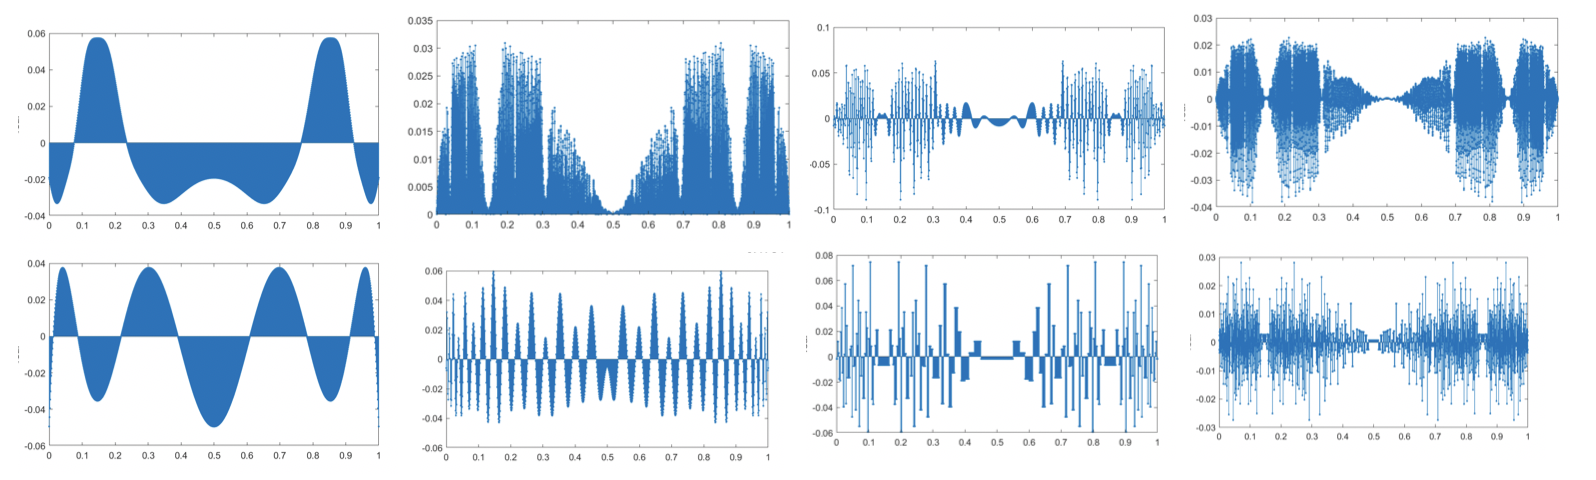
\includegraphics[width=3in]{figure/logistic_eigen_problem}
	\caption{其他的一些本征函数}
\end{figure}
\end{frame}

\begin{frame}{寻找结构简单的本征函数}
\small
\begin{itemize}
	\item $\lambda=0$的本征函数是奇异的,在本征函数中存在Jordan块结构
	\item $\lambda=0$的本征函数的线性叠加仍为本征函数,我们求得的本征函数并非最简
	\item 我们希望能够找到结构“简单”的本征函数,以更好的划分相空间
\end{itemize}
%\begin{block}{如何寻找结构简单的本征函数}
	一个显然的想法(但不见的是最好的)是构造一个我们期望的约束函数,求其最小值对应的参数,用公式可描述为$$\mathop{\arg\min}_{\boldsymbol{x},\lambda} \ \ \alpha || Ax-\lambda x || + \beta ||D(x)||_p$$
	\begin{enumerate}
		\item p:p范数
		\item $D(x)=(x_2-x_1,x_3-x_2,\cdots,x_n-x_{n-1})^T$
		\item $\alpha \gg \beta$(满足本征函数定义)
		\item 约束:$||x||\equiv 1$
	\end{enumerate}
%\end{block}
\end{frame}

\begin{frame}{Tent map的本征函数(m=4)}
\begin{figure}
	\begin{minipage}{0.2\linewidth}
		\centering
		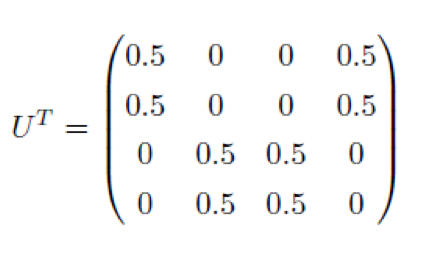
\includegraphics[width=0.8in]{figure/tent_m4_matrix}
		\caption{Koopman算符的矩阵表示(m=4)}
	\end{minipage}
	\begin{minipage}{0.6\linewidth}
		\centering
		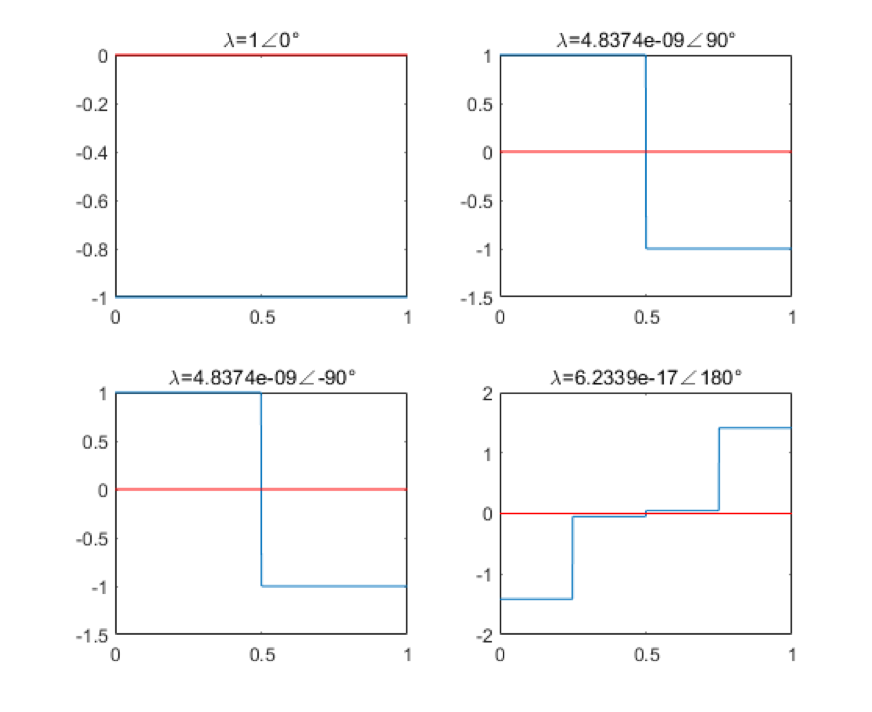
\includegraphics[width=2.8in]{figure/tent_m4_eigen}
		\caption{Tent map的本征函数}
	\end{minipage}
\end{figure}
\centering
$U^T,$ Tent map, Rectangle basis function, \textcolor{red}{m=4}
\end{frame}

\begin{frame}{Tent map的本征函数(m=100)}
\begin{figure}
	\centering
	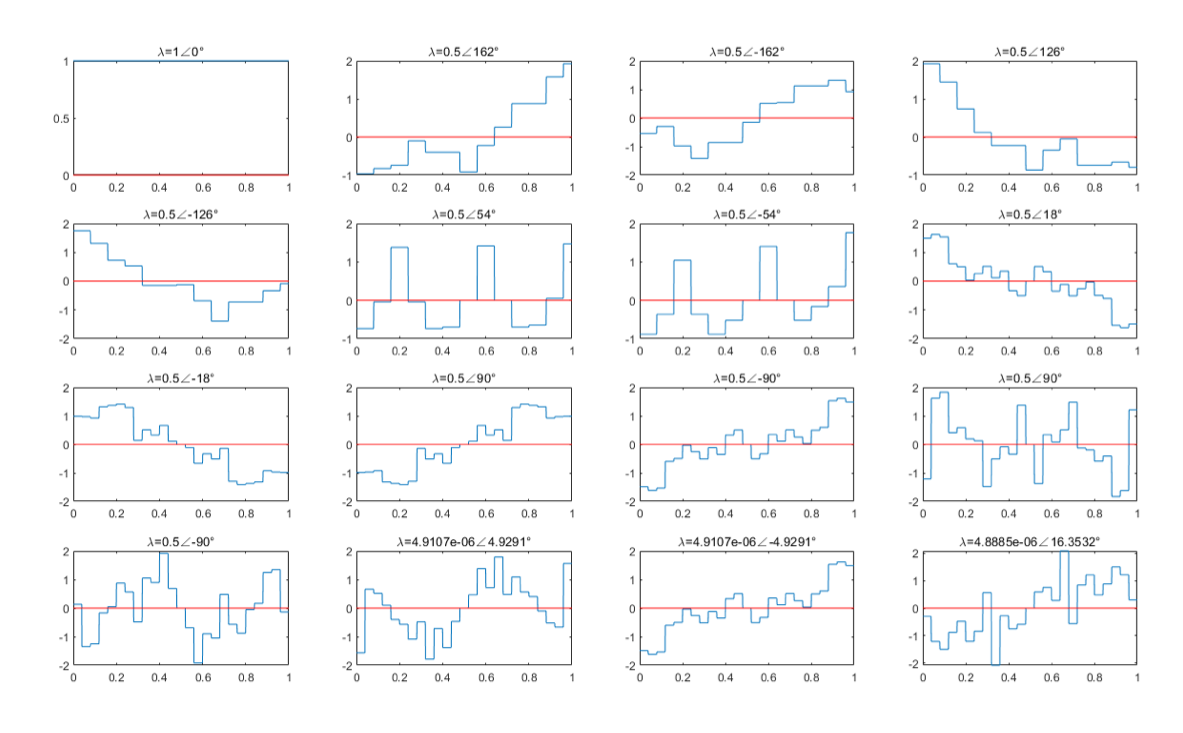
\includegraphics[width=3in]{figure/tent_eigen_m100}
	\caption{$U^T,$ Tent map, Rectangle basis function, \textcolor{red}{m=100}}
\end{figure}
\end{frame}

\begin{frame}{Tent map的本征函数(m=100)}
\begin{figure}
	\centering
	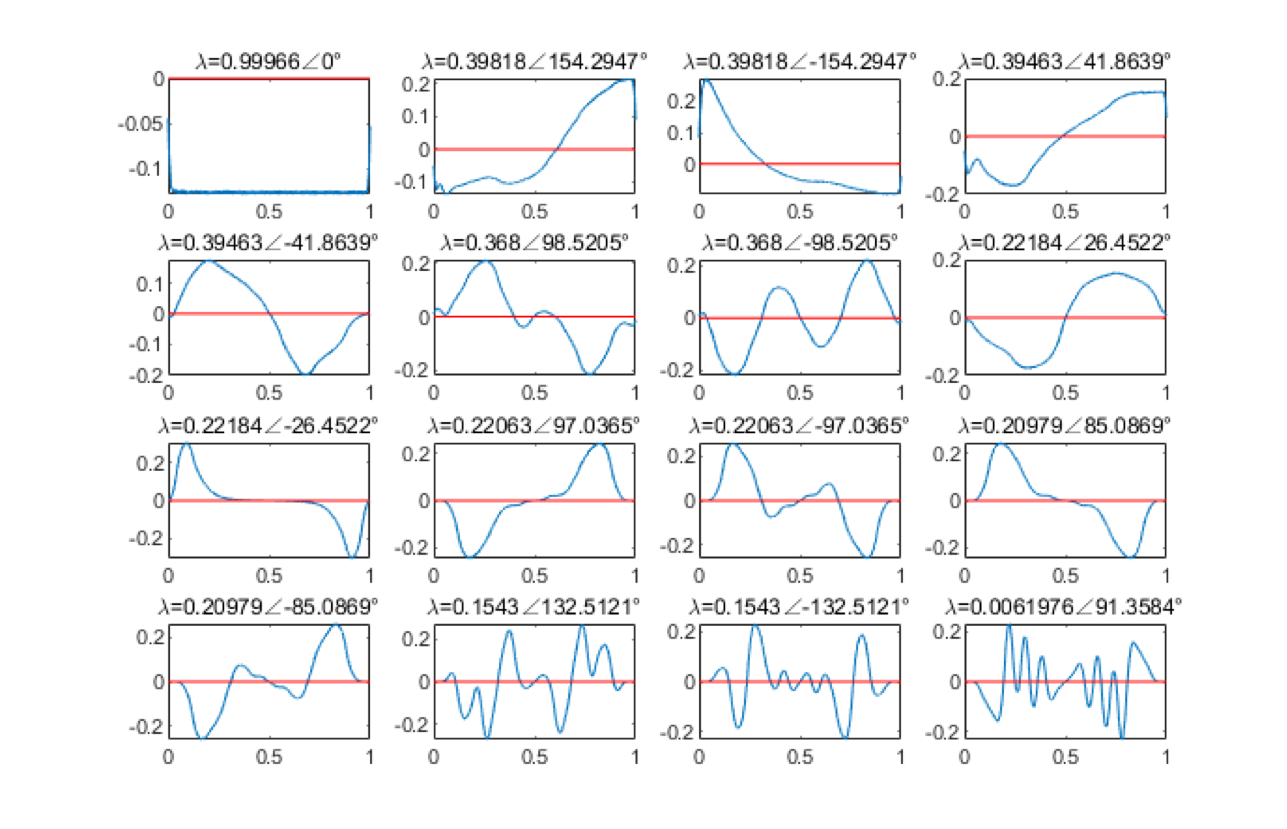
\includegraphics[width=3in]{figure/tent_eigen_gauss}
	\caption{$U^T,$ Tent map, \textcolor{red}{Gauss} basis function, m=100}
\end{figure}
\end{frame}

\begin{frame}{寻找结构简单的本征函数(迭代法)}
\begin{figure}
	\centering
	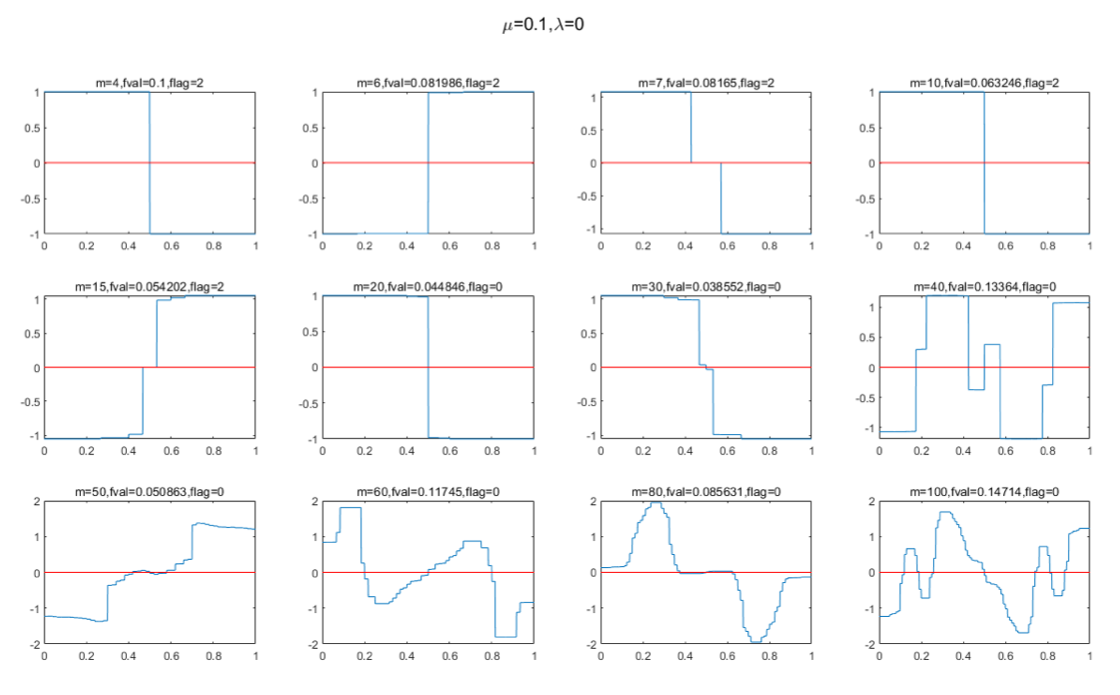
\includegraphics[width=3in]{figure/tent_iter_minimun}
	\caption{$U^T,$ Tent map, Rectangle basis function, m=[4,6,7,10,15,20,30,40,50,60,80,100]}
\end{figure}
\begin{itemize}
	\item 迭代法不能跳出局部最小值
\end{itemize}
\end{frame}

\begin{frame}{寻找结构简单的本征函数(随机梯度下降)}
\begin{figure}
	\centering
	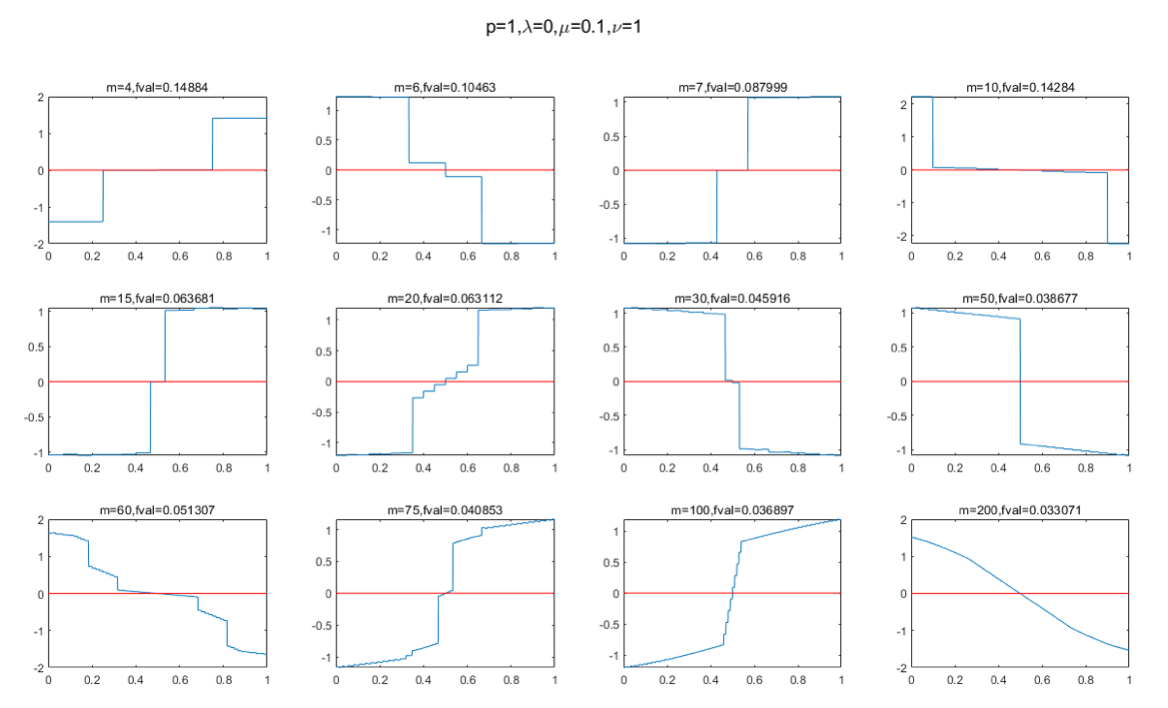
\includegraphics[width=3in]{figure/tent_svg}
	\caption{$U^T,$ Tent map, Rectangle basis function, m=[4,6,7,10,15,20,30,40,50,60,80,100]}
\end{figure}
\end{frame}

\begin{frame}{Henon map的本征函数}
\begin{figure}
	\centering
	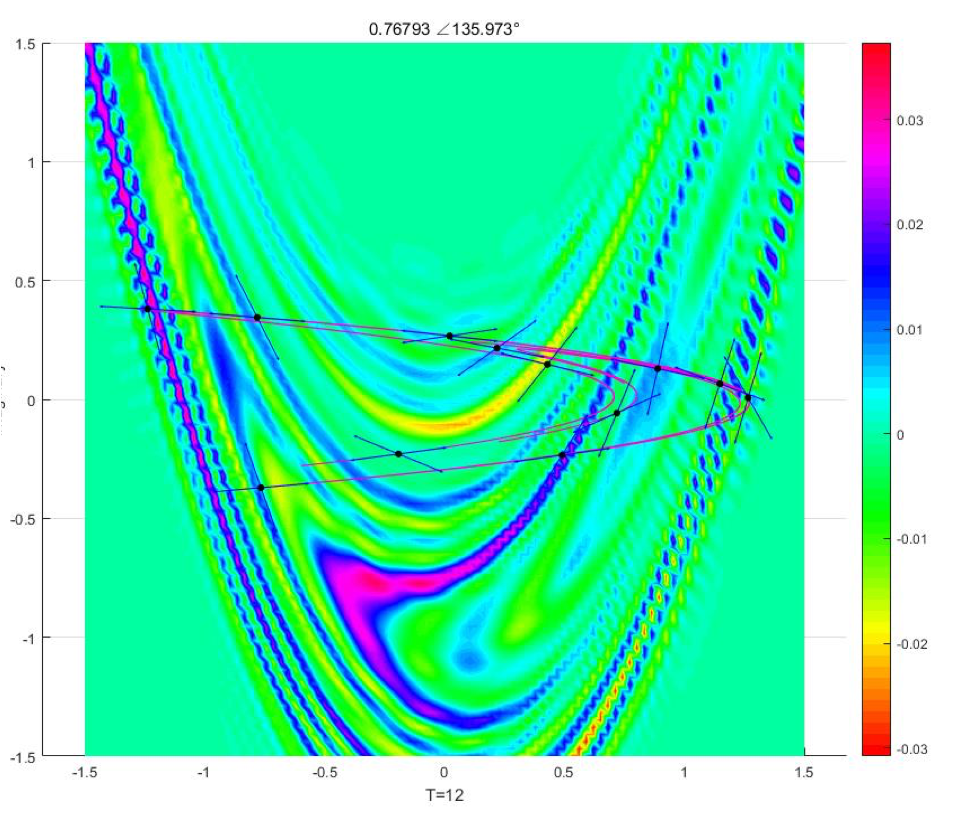
\includegraphics[width=3in]{figure/henon_eigen}
	\caption{Henon map的本征函数}
\end{figure}
Koopman算符与Henon映射的不稳定流行吻合,周期点的线性化方向(一个稳定方向,一个不稳定方向)分别与吸引子形状和本征函数一致。
\end{frame}

\begin{frame}{Henon map的本征函数}
\begin{figure}
	\centering
	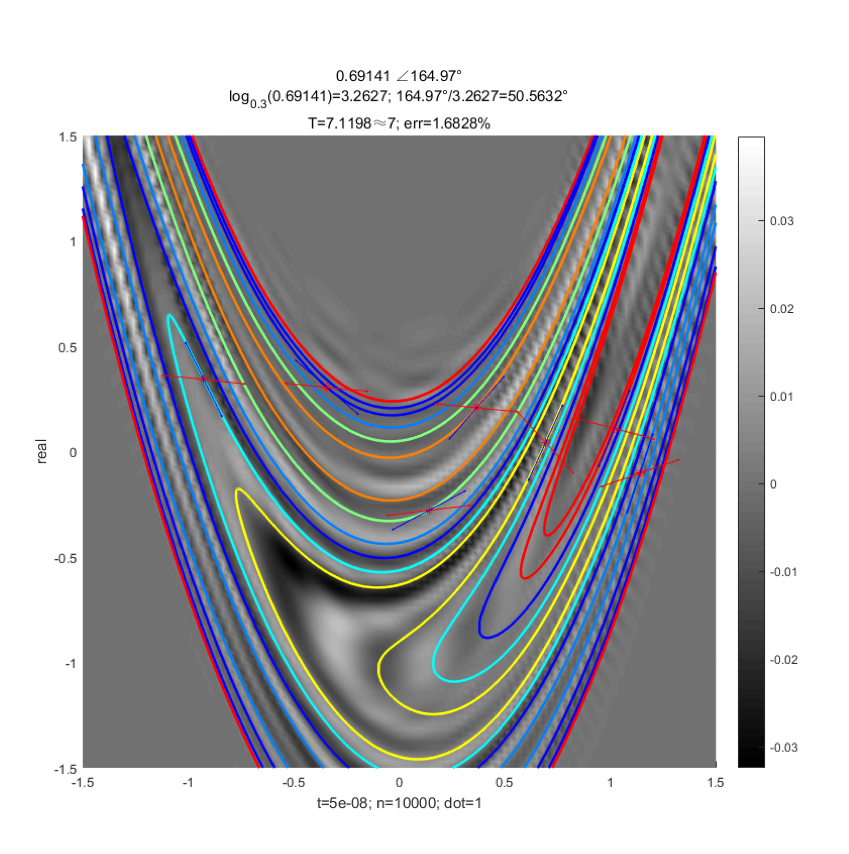
\includegraphics[width=3in]{figure/henon_evolution}
	\caption{Henon map的本征函数}
\end{figure}
Koopman算符与Henon映射的不稳定流行吻合,周期点的线性化方向(一个稳定方向,一个不稳定方向)分别与吸引子形状和本征函数一致。
\end{frame}

\begin{frame}{Lorenz System的本征函数}
\begin{figure}
	\centering
	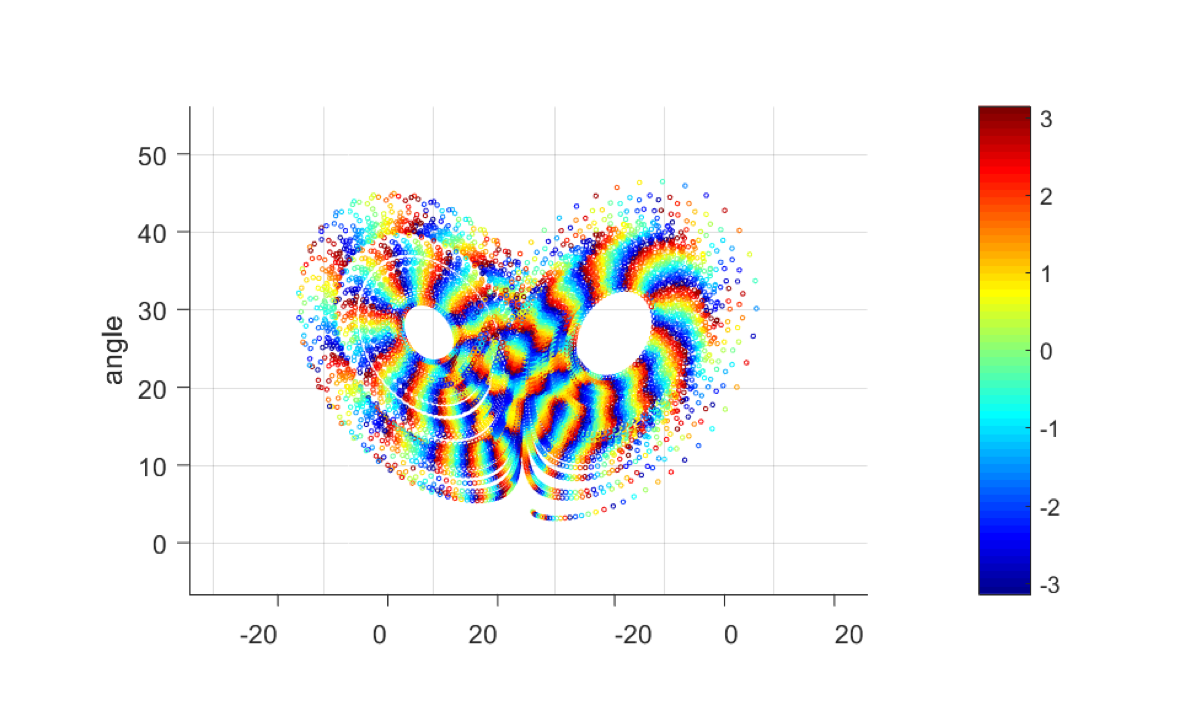
\includegraphics[width=3.5in]{figure/lorenz_eigen}
	\caption{Lorenz System的本征函数}
\end{figure}
\end{frame}

\begin{frame}{Lorenz System的本征函数}
\begin{figure}
	\centering
	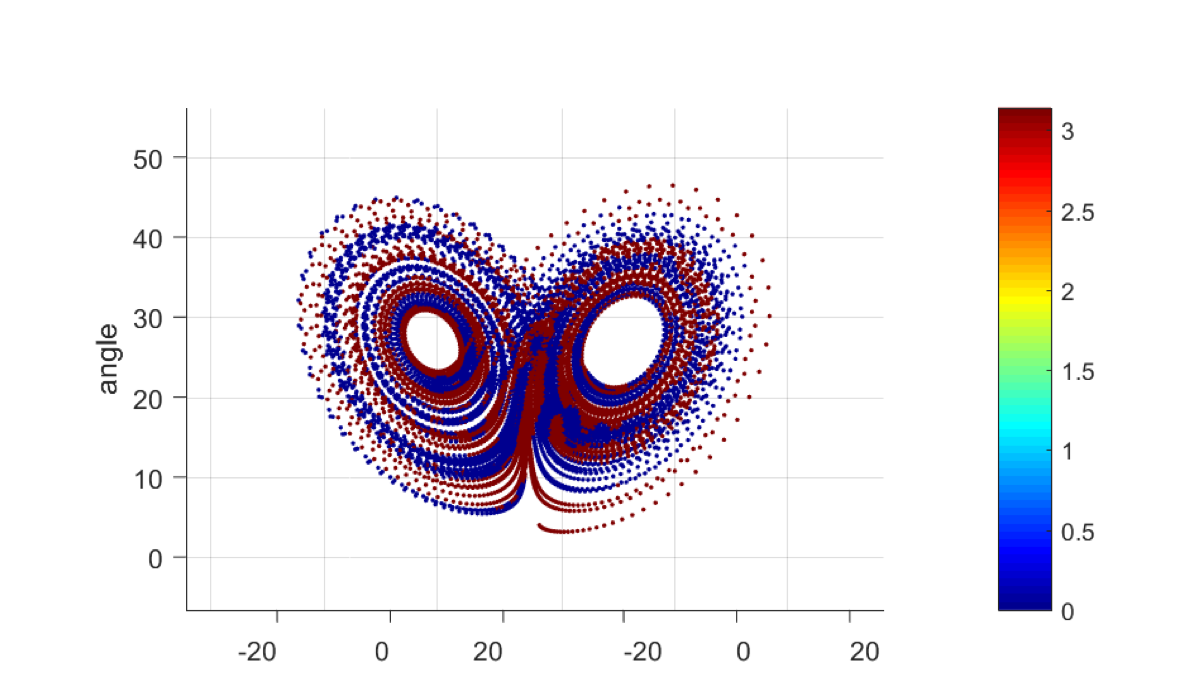
\includegraphics[width=3.5in]{figure/lorenz_eigen_bin}
	\caption{Lorenz System的本征函数}
\end{figure}
\end{frame}

\section{计划进度及安排}
\begin{frame}{计划进度及安排}
\begin{itemize}
	%\footnotesize
	\item 2017.9-2017.12
	学习非线性动力学知识,阅读相关文献;学习一般非线性系统的分析方法。
	\item 2017.12-2018.3
	查找相关文献资料,对Koopman算符的研究成果进行分析,熟悉别人对这方面做出的成果。
	\item 2018.3-2018.11
	阅读动力学系统的性质等相关书籍与文献,分析Koopman算符是如何描述动力学系统的。
	,建立初步模型并尝试仿真计算,进行模型的初步分析。
	\item 2018.11-2019.3
	阅读混沌系统与其动力学性质等相关文献,并分析混沌系统中的Koopman算符。
	写出论文提纲,对模型进一步仿真与数值计算。
	\item 2019.3-2019.9
	基于DMD对混沌系统进行Koopman分析,对得到的结果进行分析并尝试优化;开始论文的写作。
	\item 2019.9-2020.1
	优化并整理不同混沌系统中的Koopman算符的差异,对有待解决的问题进行分析;完成学位论文。
	\item 2020.1-2020.4
	对论文中存在的问题进行修改和完善;论文送审,准备答辩。
\end{itemize}
\end{frame}
\section{仍需思考并完善的问题}
\begin{frame}{仍需思考并完善的问题}
\begin{enumerate}
\item 如何精确的用一些随机梯度下降算法求得精简的本征值。以及如何跳出局部最优解。
\item 随着基函数的增多,本征函数的划分也变得更精确,如何通过粗粒度的划分来实现细粒度的划分。
\item 如果原方程加了噪声,会对Koopman算符本征函数有何影响。
\item Koopman算符的本征函数是否具有鲁棒性。
\item 如何确定边界点的层次。
\item 能否用通用的方法画出动力学系统的分界线。
\item 本征函数的最大值最小值分别表示什么含义。
\item 基函数的变化是如何影响本征函数的。
\end{enumerate}
\end{frame}
\section{参考文献}
\begin{frame}{参考文献}
\begin{itemize}
{\scriptsize
\item 贾继莹. Koopman算符在一些动力系统中的算法和应用研究[D]. 2015.
\item Brunton S L, Brunton B W, Proctor J L, et al. Chaos as an intermittently forced linear system[J]. Nature Communications, 2017, 8(1):19.
\item Strogatz S H. From Kuramoto to Crawford: exploring the onset of synchronization in populations of coupled oscillators[J]. Physica D, 2000, 143(1-4):1-20.
\item Hobson D. An Efficient Method for Computing Invariant Manifolds of Planar Maps[J]. Journal of Computational Physics, 1993, 104(1):14-22.
\item Carles Simó. On the Hénon-Pomeau attractor[J]. Journal of Statistical Physics, 1979, 21(4):465-494.
\item Pomeau Y, Berre M L. Dynamics of self-gravitating systems : Variations on a theme by Michel Henon[J]. Physics, 2014.
\item Gaspard, P. Nicolis, G. Provata, A. Tasaki, S. Spectral signature of the pitchfork bifurcation: Liouville equation. Physical Review E, 1995.
\item Gaspard P, Tasaki S. Liouvillian dynamics of the Hopf bifurcation[J]. Physical Review E, 2001, 64(5):056232.
\item Korda M, Putinar M, Mezić, Igor. Data-driven spectral analysis of the Koopman operator[J]. 2017.
\item Lan Y, Cvitanović P. Variational method for finding periodic orbits in a general flow[J]. Physical Review E, 2004, 69(1):016217.
\item Steven H. Strogatz. Nonlinear dynamics and chaos: with applications to physics, biology, chemistry, and engineering [M]. Perseus Books Publishing, 2000
\item Igor Mezić. Spectral Koopman operator in dynamical systems. Springer, 2017
}
\end{itemize}
\end{frame}
\begin{frame}{致谢}
\centering
\huge 感谢各位老师莅临指导\\[30pt]
\normalsize 北京邮电大学理学院\\
张聪
\end{frame}
\end{document}
